\documentclass{article}
\usepackage{tikz}
\usepackage{blindtext}
\usetikzlibrary{automata,positioning,arrows}
\usepackage[T1]{fontenc}
\usepackage{hyperref}
\usepackage{graphicx}
\graphicspath{.}

\title{EECS 510 Final Project}
\author{Jack Bauer}
\date{December 2024}

\begin{document}

\maketitle
\section{Part 1 - Design a Formal Language}
Inspired by some of my favorite novels, I have designed a language based on spell-casting. Spells consist of some combination of these four elements: fire, earth, air, and water. There is also a special divine element. However, for any aspiring mage, there are a few main rules to be aware of:
\begin{enumerate}
    \item 
    Fire and water are opposites, and as such they cannot appear next to each other in a valid spell. Earth and air are also opposites; they cannot appear next to each other either. 
    \item 
    Fire and earth make up the dark side. Air and water form the light side. However, light and dark must always be in balance, so there must be an equal number of light and dark elements; that is, an equal number of occurrences of fire/earth and air/water in any valid spell.
    \item 
    After extensive study, the Mages' Guild has discovered that, as fire and earth are the most foundational elements, they must come first in any valid spell.
    \item Since all magic comes from the Gods, mages must mind their ps and qs and start and end each spell with a please and a thank you. 
    \item Additionally, a new element has recently been discovered, the divine element, that connects you directly with the Gods. However, it must be cast on its own, without any light or dark elements (while maintaining the respectful ps and qs of course). One may address as many Gods as they wish, and thus cast this divine element an unlimited number of times. 
    \item Also, one cannot just say please and thank you. There's no point in being polite if one doesn't want anything. Do not be over-polite, one please and thank you is enough; any more would annoy the Gods. 
    \item
    Finally, nothing is not a valid spell. There's no magic in the absence of magic, right? 
\end{enumerate}
For more details, see below. Fire is represented as f, air as a, water as w, and earth as e. Respect at the start and end of spells is represented with p and q. The stand-alone magical element of the Gods is represented with a g. If you learn these rules, you will become more powerful than you can imagine!
\begin{center}
    $\Sigma$ = \{p, f, e, a, w, g, q\}\\
    $\Gamma$ = \{X, Y\} \\
    \hfill \\ 
\end{center}
Rules
\begin{itemize}
    \item f and w cannot follow each other.
    \item a and e cannot follow each other.
    \item D = \{f, e\} and L = \{a, w\}. There must be an equal number of elements from L and D. 
    \item All elements from D must precede all elements from L. 
    \item All strings must start with p and end with q. However, pq is not a valid string. There may only be one p and one q in a string.
    \item If g appears in a string, only g may appear in that string.
    \item $\lambda$ is not a valid string.
    \end{itemize}
Some example valid strings: pfffeeewaaawawq, pfaq, pewq, peefewaawq, pgq, .
\section{Part 2 - Grammar}
The grammar of this language is context-free. It is as follows:
\begin{center}
    $S \rightarrow$ pXq | pgYq \\
    $Y \rightarrow$ gY | $\lambda$ \\
    $X \rightarrow$ T | DXL \\
    $L\rightarrow$ a | w\\
    $D \rightarrow$ f | e \\
    $T \rightarrow$ fa | ew
\end{center}
\newpage
\section{Part 3 - Automaton}
Definitions: 
\begin{center}
    \begin{itemize}
        \item Q = \{$q_s$, $q_p$, $q_g$, $q_f$, $q_e$, $q_a$, $q_w$, $q_q$,\}
        \item $\delta$ =\\ $\{
        ((q_s,p, \lambda), (q_p,Y)),$\\
        $((q_p,f, \lambda), (q_f,X)),
        ((q_p,g, \lambda), (q_g,\lambda)),
        ((q_p,e, \lambda), (q_e,X)),$\\
        $((q_g, g, \lambda), (q_g, \lambda))
        ((q_g, q, Y), (q_q, \lambda))$\\
        $((q_f,f, \lambda), (q_f,X)),
        ((q_f,a, X), (q_a,\lambda)),
        ((q_f,e, \lambda), (q_e,X))$\\
        $((q_e,e, \lambda), (q_e,X)),
        ((q_e,w, X), (q_w,\lambda)),
        ((q_e,f, \lambda), (q_f,X)),$\\
        $((q_w,a, X), (q_a,\lambda)),
        ((q_w,w, X), (q_w,\lambda)),
        ((q_w,q, Y), (q_q,\lambda)),$\\
        $((q_a,a, X), (q_a,\lambda)),
        ((q_a,w, X), (q_w,\lambda))
        ((q_a,q, Y), (q_q,\lambda)),
        \}$
    \end{itemize}
\end{center}
For the PDA, see Figure 1.
\begin{figure}
    \centering
    \begin{tikzpicture}[shorten >= 1pt, node distance=2cm,on grid,auto, scale=.8, transform shape]
    \node[state,initial] (q_s) at (-8.5, 0) {$q_s$};
    \node[state] (q_p) at (-5.5, 0) {$q_p$};
    \node[state] (q_g) at (-5.5, 5) {$q_g$};
    \node[state] (q_f) at (-2, 3) {$q_f$};
    \node[state] (q_a) at (3, 3) {$q_a$};
    \node[state] (q_w) at (3, -3) {$q_w$};
    \node[state,accepting] (q_q) at (6.5, 0) {$q_q$};
    \node[state] (q_e) at (-2, -3) {$q_e$};
    \path[->]
    (q_s) edge node {p, $\lambda$ $\rightarrow$ Y} (q_p)
    (q_g) edge [loop above] node {g, $\lambda$ $\rightarrow$ $\lambda$} (q_g)
          edge [bend left=80, looseness=.9] node {q, Y $\rightarrow$ $\lambda$} (q_q)
    (q_p) edge node {f, $\lambda$ $\rightarrow$ X} (q_f)
          %edge [bend right=80, looseness=1.5] node [swap] {W, $\lambda$ $\rightarrow$ L} (q_w)
          %edge node [swap] {A, $\lambda$ $\rightarrow$ L} (q_a)
          edge [swap] node {e, $\lambda$ $\rightarrow$ X} (q_e)
          edge node {g, $\lambda$ $\rightarrow$ $\lambda$} (q_g)
    (q_f) %edge [loop above] node {F, L $\rightarrow$ D} ()
          edge [loop above] node [] {f, $\lambda$ $\rightarrow$ X} ()
          %edge [bend left=20] node {E, L $\rightarrow$ D} (q_e)
          edge [bend left=20] node {e, $\lambda$ $\rightarrow$ X} (q_e)
          edge node {a, X $\rightarrow$ $\lambda$} (q_a)
          %edge [bend left=20] node [yshift=-.4cm] {A, $\lambda$ $\rightarrow$ L} (q_a)
    (q_e) %edge [loop below] node {E, L $\rightarrow$ D} ()
          edge [loop below] node {e, $\lambda$ $\rightarrow$ X} ()
          %edge [bend left=20] node {E, L $\rightarrow$ D} (q_f)
          edge [bend left=20] node {f, $\lambda$ $\rightarrow$ X} (q_f)
          edge node {w, X $\rightarrow$ $\lambda$} (q_w)
          %edge [] node [yshift=-.4cm] {W, $\lambda$ $\rightarrow$ L} (q_w)
    (q_w) edge [loop below] node [xshift=.4cm] {w, X $\rightarrow$ $\lambda$} ()
          %edge [loop below] node [below=of q_w, yshift=1.3cm, xshift=.4cm] {W, $\lambda$ $\rightarrow$ L} ()
          edge [bend left=20] node {a, X $\rightarrow$ $\lambda$} (q_a)
          %edge [bend left=20] node [yshift=-.4cm] {A, $\lambda$ $\rightarrow$ L} (q_a)
          %edge [bend left=20] node {E, L $\rightarrow$ D} (q_e)
          %edge [bend left=20] node [yshift=-.4cm] {E, $\lambda$ $\rightarrow$ D} (q_e)
          edge node [swap] {q, Y $\rightarrow$ $\lambda$} (q_q)
    (q_a) edge [loop above] node {a, X $\rightarrow$ $\lambda$} ()
          %edge [loop below] node [below=of q_a, yshift=1.3cm] {A, $\lambda$ $\rightarrow$ L} ()
          edge [bend left=20] node {w, X $\rightarrow$ $\lambda$} (q_w)
          edge node {q, Y $\rightarrow$ $\lambda$} (q_q);
          %edge [bend left=20] node [yshift=.4cm] {W, $\lambda$ $\rightarrow$ L} (q_w)
          %edge [bend left=20] node {F, L $\rightarrow$ D} (q_f)
          %edge [bend left=20] node [yshift=-.4cm] {F, $\lambda$ $\rightarrow$ D} (q_f);
    \end{tikzpicture}
    \caption{The PDA for the Elemental Language}
    \label{fig:enter-label}
\end{figure}
\newpage
\section{Part 4 - Data Structure}
The data structure for this language is stored as a file in memory. The file format is as follows:\\
- Line 1: A whitespace-delimited list of states.\\
- Line 2: A whitespace-delimited list of input symbols. \\
- Line 3: A whitespace-delimited list of stack symbols. \\
- Line 4: The start state. \\
- Line 5: A whitespace-delimited list of accepting states. \\
- Lines 6-23: Each line is a whitespace-delimited list of elements representing a transition, in the following order:
\begin{enumerate}
    \item The beginning state of the transition.
    \item The input character.
    \item The ending state of the transition.
    \item The stack variable popped. An \_ represents $\lambda$.
    \item The stack variable pushed. An \_ represents $\lambda$. 
\end{enumerate}
Using this format, the automaton can be represented as a text file with the following 23 lines:
\begin{enumerate}
    \item q\_s q\_p q\_g q\_f q\_e q\_w q\_a q\_q
    \item p g a e f w q
    \item X Y
    \item q\_s
    \item q\_q
    \item q\_s p q\_p \_ Y
    \item q\_p g q\_g \_ \_
    \item q\_p f q\_f \_ X
    \item q\_p e q\_e \_ X
    \item q\_g g q\_g \_ \_
    \item q\_g q q\_q Y \_
    \item q\_f f q\_f \_ X
    \item q\_f e q\_e \_ X
    \item q\_f a q\_a X \_
    \item q\_e f q\_f \_ X
    \item q\_e e q\_e \_ X
    \item q\_e w q\_w X \_
    \item q\_a a q\_a X \_
    \item q\_a w q\_w X \_
    \item q\_a q q\_q Y \_
    \item q\_w a q\_a X \_
    \item q\_w w q\_w X \_
    \item q\_w q q\_q Y \_
\end{enumerate}

\section{Part 5 - Testing}
The code to test strings for the automaton is located here:
\url{https://github.com/bribedjupiter/eecs510_final_project}. There is a file, main.py, that when ran will ask the user for an input string. It will then load the automaton from automaton.txt, represented using the data structure from Part 4, and then call a function to check if the automaton accepts the input string. If it accepts, then it will list the steps it took while processing the string. If it rejects, it will simply say reject. It is also possible that it may raise an error, but if it does it could be the result of a malformed input file. Here are some sample outputs:
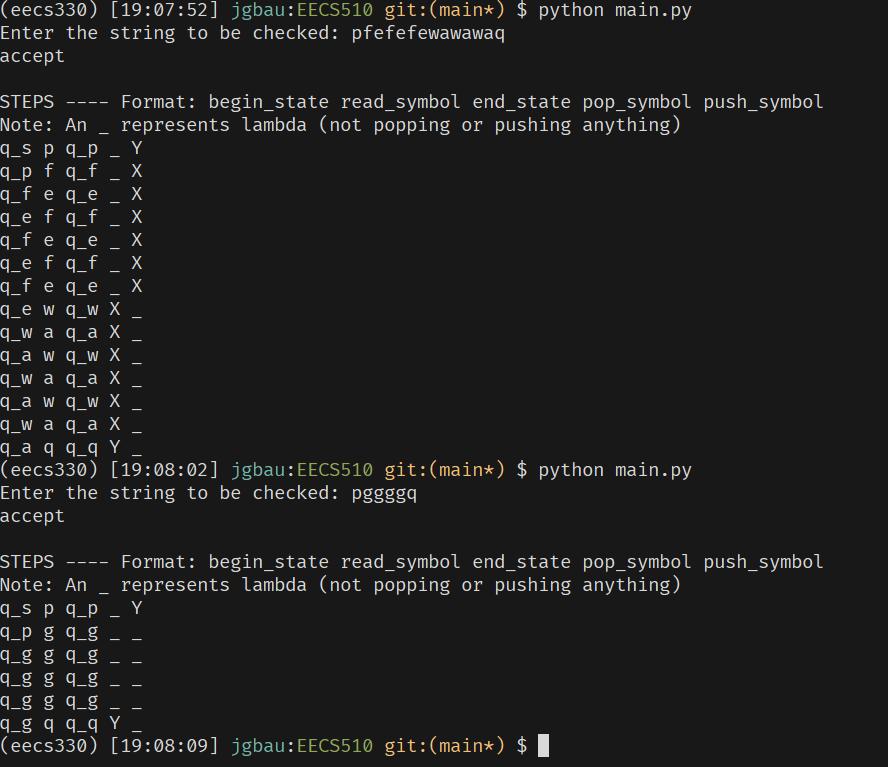
\includegraphics[width=\textwidth]{part5-accept.png}
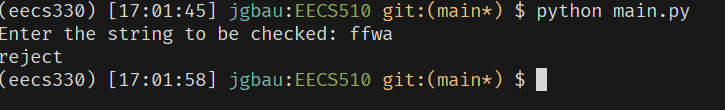
\includegraphics[width=\textwidth]{part5-reject.png}
\end{document}
